\documentclass[journal,12pt,twocolumn]{IEEEtran}

\usepackage{setspace}
\usepackage{gensymb}

\singlespacing


\usepackage[cmex10]{amsmath}

\usepackage{amsthm}

\usepackage{mathrsfs}
\usepackage{txfonts}
\usepackage{stfloats}
\usepackage{bm}
\usepackage{cite}
\usepackage{cases}
\usepackage{subfig}

\usepackage{longtable}
\usepackage{multirow}

\usepackage{enumitem}
\usepackage{mathtools}
\usepackage{steinmetz}
\usepackage{tikz}
\usepackage{circuitikz}
\usepackage{verbatim}
\usepackage{tfrupee}
\usepackage[breaklinks=true]{hyperref}
\usepackage{graphicx}
\usepackage{tkz-euclide}
\usepackage{float}

\usetikzlibrary{calc,math}
\usepackage{listings}
\usepackage{color} %%
\usepackage{array} %%
\usepackage{longtable} %%
\usepackage{calc} %%
\usepackage{multirow} %%
\usepackage{hhline} %%
\usepackage{ifthen} %%
\usepackage{lscape}
\usepackage{multicol}
\usepackage{chngcntr}

\DeclareMathOperator*{\Res}{Res}

\renewcommand\thesection{\arabic{section}}
\renewcommand\thesubsection{\thesection.\arabic{subsection}}
\renewcommand\thesubsubsection{\thesubsection.\arabic{subsubsection}}

\renewcommand\thesectiondis{\arabic{section}}
\renewcommand\thesubsectiondis{\thesectiondis.\arabic{subsection}}
\renewcommand\thesubsubsectiondis{\thesubsectiondis.\arabic{subsubsection}}


\hyphenation{op-tical net-works semi-conduc-tor}
\def\inputGnumericTable{} %%

\lstset{
%language=C,
frame=single,
breaklines=true,
columns=fullflexible
}
\begin{document}


\newtheorem{theorem}{Theorem}[section]
\newtheorem{problem}{Problem}
\newtheorem{proposition}{Proposition}[section]
\newtheorem{lemma}{Lemma}[section]
\newtheorem{corollary}[theorem]{Corollary}
\newtheorem{example}{Example}[section]
\newtheorem{definition}[problem]{Definition}

\newcommand{\BEQA}{\begin{eqnarray}}
\newcommand{\EEQA}{\end{eqnarray}}
\newcommand{\define}{\stackrel{\triangle}{=}}
\bibliographystyle{IEEEtran}
\providecommand{\mbf}{\mathbf}
\providecommand{\pr}[1]{\ensuremath{\Pr\left(#1\right)}}
\providecommand{\qfunc}[1]{\ensuremath{Q\left(#1\right)}}
\providecommand{\sbrak}[1]{\ensuremath{{}\left[#1\right]}}
\providecommand{\lsbrak}[1]{\ensuremath{{}\left[#1\right.}}
\providecommand{\rsbrak}[1]{\ensuremath{{}\left.#1\right]}}
\providecommand{\brak}[1]{\ensuremath{\left(#1\right)}}
\providecommand{\lbrak}[1]{\ensuremath{\left(#1\right.}}
\providecommand{\rbrak}[1]{\ensuremath{\left.#1\right)}}
\providecommand{\cbrak}[1]{\ensuremath{\left\{#1\right\}}}
\providecommand{\lcbrak}[1]{\ensuremath{\left\{#1\right.}}
\providecommand{\rcbrak}[1]{\ensuremath{\left.#1\right\}}}
\theoremstyle{remark}
\newtheorem{rem}{Remark}
\newcommand{\sgn}{\mathop{\mathrm{sgn}}}
\providecommand{\abs}[1]{\left\vert#1\right\vert}
\providecommand{\res}[1]{\Res\displaylimits_{#1}}
\providecommand{\norm}[1]{\left\lVert#1\right\rVert}
%\providecommand{\norm}[1]{\lVert#1\rVert}
\providecommand{\mtx}[1]{\mathbf{#1}}
\providecommand{\mean}[1]{E\left[ #1 \right]}
\providecommand{\fourier}{\overset{\mathcal{F}}{ \rightleftharpoons}}
%\providecommand{\hilbert}{\overset{\mathcal{H}}{ \rightleftharpoons}}
\providecommand{\system}{\overset{\mathcal{H}}{ \longleftrightarrow}}
%\newcommand{\solution}[2]{\textbf{Solution:}{#1}}
\newcommand{\solution}{\noindent \textbf{Solution: }}
\newcommand{\cosec}{\,\text{cosec}\,}
\providecommand{\dec}[2]{\ensuremath{\overset{#1}{\underset{#2}{\gtrless}}}}
\newcommand{\myvec}[1]{\ensuremath{\begin{pmatrix}#1\end{pmatrix}}}
\newcommand{\mydet}[1]{\ensuremath{\begin{vmatrix}#1\end{vmatrix}}}
\numberwithin{equation}{subsection}
\makeatletter
\@addtoreset{figure}{problem}
\makeatother
\let\StandardTheFigure\thefigure
\let\vec\mathbf
\renewcommand{\thefigure}{\theproblem}
\def\putbox#1#2#3{\makebox[0in][l]{\makebox[#1][l]{}\raisebox{\baselineskip}[0in][0in]{\raisebox{#2}[0in][0in]{#3}}}}
\def\rightbox#1{\makebox[0in][r]{#1}}
\def\centbox#1{\makebox[0in]{#1}}
\def\topbox#1{\raisebox{-\baselineskip}[0in][0in]{#1}}
\def\midbox#1{\raisebox{-0.5\baselineskip}[0in][0in]{#1}}
\vspace{3cm}
\title{Assignment No.1} 
\author{Suyog Tangade\\MD/2020/710} 
\maketitle
\newpage
\bigskip
\renewcommand{\thefigure}{\theenumi}
\renewcommand{\thetable}{\theenumi}
Download all python codes from
\begin{lstlisting}
https://github.com/suyogtangade/AI.git
\end{lstlisting}
%
and latex-tikz codes from
%
\begin{lstlisting}
https://github.com/suyogtangade/AI.git
\end{lstlisting}
%
\section{Question No.16(b) (cbse/2006/set-2)}

Find the co-ordinates of the point equidistant from three given points $\vec{A}\myvec{5\\3}$, $\vec{B}\myvec{5\\-5}$ and $\vec{C}\myvec{1\\-5}$ 
\solution

Let the point equidistant from $\Vec{A}$ \& $\Vec{B}$ \& $\Vec{C}$ be 
\begin{align}
    \Vec{P}=\myvec{x\\y}
\end{align}
From the given information 
\begin{align}
    \norm{\Vec{P}-\vec{A}}^2 &= \norm{\vec{P}-\vec{B}}^2 = \norm{\vec{P}-\vec{C}}^2\\
\therefore
    \norm{\Vec{P}-\vec{A}}^2 &= \norm{\vec{P}-\vec{B}}^2
\end{align}
\begin{align}
    \norm{\vec{P}-\myvec{5\\3}}^2 =\norm{\vec{P} - \myvec{5\\-5}}^2
    \end{align}
    \begin{align}
    \norm{\vec{P}}^2 + \norm{\vec{A}}^2 -2\vec{A}^T\vec{P} = \norm{\vec{P}}^2 + \norm{\vec{B}}^2 -2\vec{B}^T\vec{P}
\end{align}
\begin{align} 
    \Longrightarrow \norm{\vec{P}}^2 + \norm{\myvec{5\\3}}^2 -2\vec{A}^T\vec{P}\\ = \norm{\vec{P}}^2 + \norm{\myvec{5\\-5}}^2 -2\vec{B}^T\vec{P}
\end{align}
\begin{align}
    \norm{\myvec{5\\3}}^2 -\norm{\myvec{5\\-5}}^2 \\= 2\myvec{5& 3}\vec{P} -2\myvec{5&-5}\vec{P}
    \end{align}
    \begin{align}
    \myvec{\sqrt{5^2}+\sqrt{3^2}} -\myvec{\sqrt{5^2}+\sqrt{-5^2}} \\=                  \bigg[\myvec{10&6} - \myvec{10&-10}\bigg]\vec{P}
\end{align}
\begin{align}
    \myvec{\sqrt{34}} -\myvec{\sqrt{50}}                      =\bigg[\myvec{16&0}\bigg]\vec{P}
\end{align}
\begin{align}
    \vec{-16} = \myvec{16&0}\vec{P}
\end{align}
Which can be simplified to obtain 
\begin{align}
    \myvec{0&16}\vec{P} = -16
    \Longrightarrow y = -1
\end{align}
\begin{align}
    \norm{\vec{P}}^2 + \norm{\vec{B}}^2 -2\vec{B}^T\vec{P} \\= \norm{\vec{P}}^2 + \norm{\vec{C}}^2 -2\vec{C}^T\vec{P}
\end{align}
\begin{align}
    \norm{\vec{B}}^2 - \norm{\vec{C}}^2 =2\vec{B}^T\vec{P} -2\vec{C}^T\vec{P}
\end{align}
\begin{align}
    \norm{\vec{P}-\myvec{5\\-5}}^2 =\norm{\vec{P} - \myvec{1\\-5}}^2\\
    \Longrightarrow \norm{\vec{P}}^2 + \norm{\myvec{5\\-5}}^2 -2\vec{B}^T\vec{P}\\ = \norm{\vec{P}}^2 + \norm{\myvec{1\\-5}}^2 -2\vec{C}^T\vec{P}
\end{align}
\begin{align}
    \norm{\myvec{5\\-5}}^2 -2\vec{B}^T\vec{P} = \norm{\myvec{1\\-5}}^2 -2\vec{C}^T\vec{P}
\end{align}
\begin{align}
    \myvec{\sqrt{5^2}+\sqrt{-5^2}} -2\myvec{5&-5}\vec{P} \\= \myvec{\sqrt{1^2}+\sqrt{-5^2}} -2\myvec{1&-5}\vec{P}         
\end{align}
\begin{align}
    \myvec{\sqrt{25}+\sqrt{25}} -\myvec{-10&10}\vec{P} \\= \myvec{\sqrt{1}+\sqrt{25}} -\myvec{-2&10}\vec{P}
\end{align}
\begin{align}
    \myvec{\sqrt{50}} -\myvec{-10&10}\vec{P} \\= \myvec{\sqrt{26}} -\myvec{-2&10}\vec{P}
\end{align}
\begin{align}
    24 = \myvec{0&8}\vec{P}
\end{align}
Which can be simplified to obtain
\begin{align}
    \myvec{8&0}\vec{P} = 24
    \Longrightarrow x = 3
\end{align}
The required point 
\begin{align}
    \vec{P}=\myvec{3\\-1}.
\end{align}
\numberwithin{figure}{section}
\begin{figure}
    \centering
    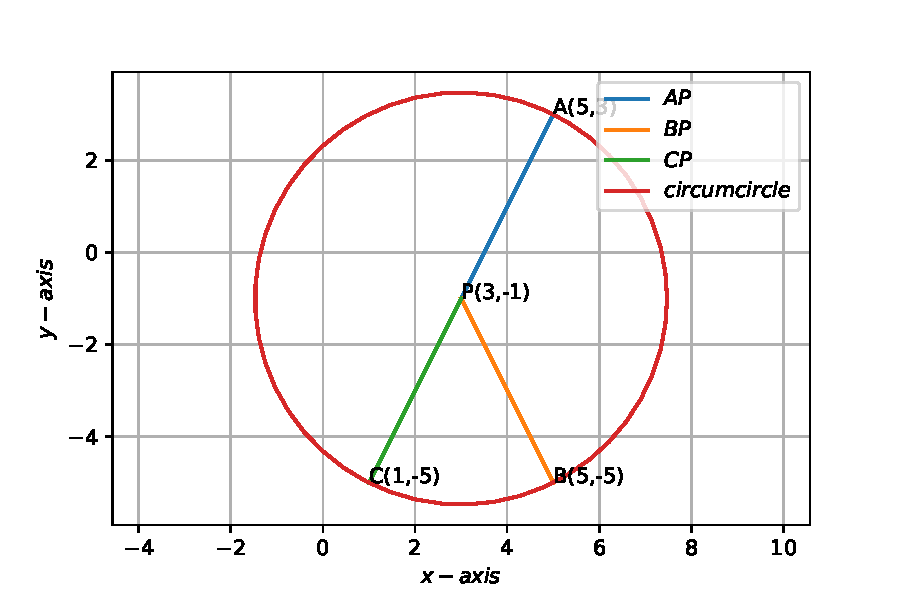
\includegraphics[width=\columnwidth]{equidistant point circumcircle.pdf}
    \caption{Graphical Solution}
    \label{fig:my_label}
\end{figure}\\
\end{document}

